%%%%%%%%%%%%%%%%%%%%%%%%%%%%%%%%%%%%%%%%%%%%%%%%%%%%%%%%%%%%%%%%%%%%%%%%
% Preamble
%%%%%%%%%%%%%%%%%%%%%%%%%%%%%%%%%%%%%%%%%%%%%%%%%%%%%%%%%%%%%%%%%%%%%%%%
\documentclass[11pt]{article}
%
% Packages and other includes
% Pagination
\usepackage[letterpaper, margin=1.25in]{geometry}
%
% Fonts
\usepackage[T1]{fontenc} % best for Western European languages
\usepackage{lmodern} % Latin Modern instead of CM
\usepackage{textcomp} % required to get special symbols
%
% Math
\usepackage{amsmath, amssymb}
\usepackage{braket}
%
% Graphics, floats, tables
\usepackage{graphicx, xcolor, float, array}
\usepackage{subcaption}
%
% Hyperlinks
\usepackage{hyperref}
%
% Bibliography
\usepackage[style=numeric, sorting=none, backend=biber]{biblatex}
\addbibresource{references.bib}
%
% Revision (see Makefile)
%\input{revision.tex}
%
% Definitions and settings
% Paragraph indent and spacing
\setlength{\parskip}{0.4\baselineskip}
\setlength{\parindent}{0in}
%
% Math mode version of "r" column type (requires array package)
\newcolumntype{R}{>{$}r<{$}}
%
%comments
\newcommand{\brian}[1]{{\color{orange} #1}}
% Title, authors, date
\title{\textbf{Is Using TPSS and TPSSh for RPA better for noncovalent
    calculations?}}
\author{Thanh Huynh and Brian Nguyen}
\date{11/27/2020 -- 01/10/2021 }
%
%
%%%%%%%%%%%%%%%%%%%%%%%%%%%%%%%%%%%%%%%%%%%%%%%%%%%%%%%%%%%%%%%%%%%%%%%%
% Main document
%%%%%%%%%%%%%%%%%%%%%%%%%%%%%%%%%%%%%%%%%%%%%%%%%%%%%%%%%%%%%%%%%%%%%%%%
%

\begin{document}

\maketitle

\section{Introduction}

Cytotoxic natural products derived from the sea squirt can be useful in cancer
therapeutics or other pharmaceuticals, such as medication
for COVID-19. In cancer treatments, the cyotoxin called chlorolissoclimide induces cell death
by inhibiting translation. Chlorolissoclimide binds to the 80S eukaryotic
ribosome to obstruct the production of proteins. An interesting ribosome-drug
interaction was revealed to form a halogen-$\pi$ bond however,
characteristics of the bond are still unknown. These interactions fall in
the category of halogen bonds. These bonds are noncovalent interactions that
are formed when an electrophilic region of the halogen in a molecule interacts
with a nucleophilic region within another molecule. It forms a $\sigma$-hole
interaction. Research in this specific interaction could help with creating
new cancer therapeutic or improving medication.

Following up with the previous report, random phase approximation (RPA) was
chosen to predict the halogen-$\pi$ interaction because RPA provides a
systematic approach to treating long-range interactions albiet, it may
not be as accurate with Grimme dispersion corrections for some cases. In addition to
these conclusions, we investigated the use of different density functional
approximations (DFAs) for RPA calculations, denoted as RPA(DFA).
The TPSS and TPSSh functionals may describe the halogen-$\pi$ bond more accurately
than PBE and investigated. To determine which functional performs better,
the X40 test set serves as a benchmark for RPA(TPSS), RPA(TPSSh), and
RPA(PBE) calculations. Moreover, the def2-QZVP basis sets were
included to determine whether it may provide a balance between efficiency
and accuracy.

\section{Methods}

Based on the previous report, the 3-4 extrapolation of the RPA
correlation energy was a good balance between efficiency and accuracy.
The X40 Test Set was used to benchmark the method's accuracy for 
noncovalent interactions involving halogens. The test set contains 40
complexes with despersion, induction, dipole-dipole, stack, hydrogen
bond, halogen bond, and halogen-$\pi$ bond interations.

To conserve time, a set of eight complexes from the X40 test set were
chosen based on error from the previous report to study basis set
convergences. A comparison of density functionals was done between
PBE, TPSS, and TPSSh. All calculations were computed with basis sets def2-QZVP,
cc-pVTZ, and cc-pVQZ to compare effects of the basis sets. Within the frozen core approximation,
the RPA energies were computed based on converged orbitals from TPSS and TPSSh, and
resolution-of-identity (RI) was included to improve efficiency. The Hartree
Exact Exchange (HXX) total energy and RIRPA correlation energy were
recorded from the supermolecule and monomers of each complex to compute
interaction energies. The interaction energies from the selected complexes
were extrapolated using the supramolecular approach. Due to the basis set
superposition error (BSSE), 50$\%$ counterpoise corrections (CP) were
applied to the RIRPA correlation energy as well. Statistical analysis
is provided.

\section{Results}

\subsection{Differences in Basis Sets}

\begin{figure}[hbpt]
  \centering
  \begin{subfigure}{\textwidth}
    \center
    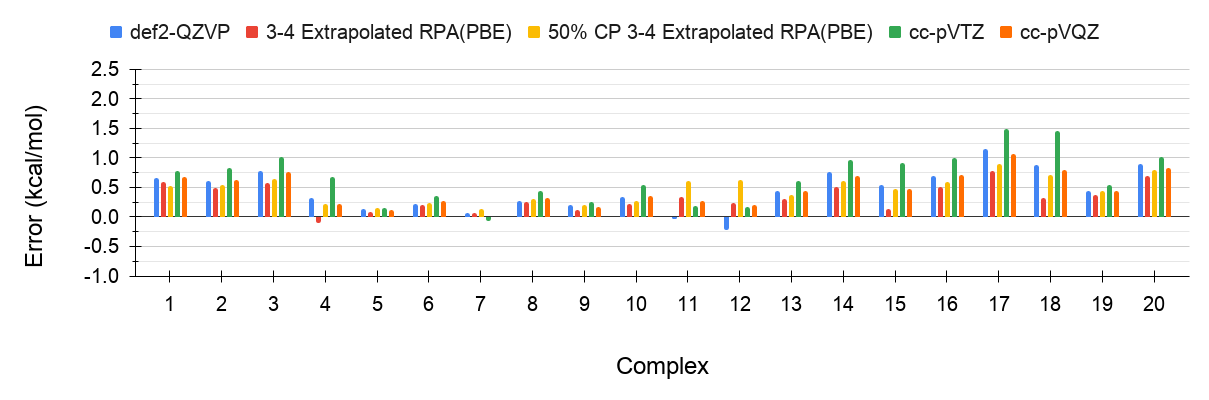
\includegraphics[scale=0.35]{def2-QZVP_1.png}
    \label{fig:def2-QZVP_1}
  \end{subfigure}
  \begin{subfigure}{\textwidth}
    \center
    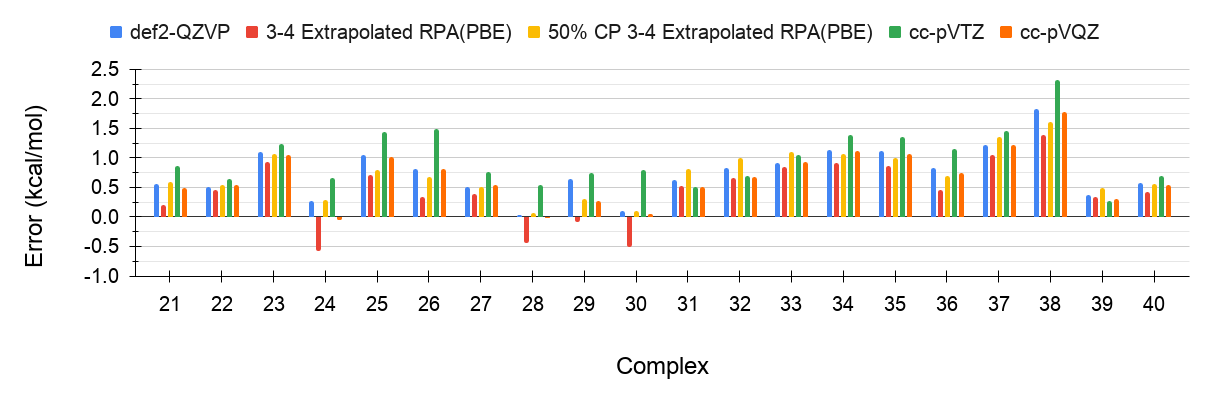
\includegraphics[scale=0.35]{def2-QZVP_2.png}
    \label{fig:def2-QZVP_2}
  \end{subfigure}
  \caption{The binding energy errors (kcal/mol) for X40 test set computed
    for RPA(PBE) methods with basis functions def2-QZVP, cc-pVTZ, and
    cc-pVQZ. Negative sign indicates overbinding.}
  \label{fig:def2-QZVP Error}
\end{figure}

For most complexes in Fig. \ref{fig:def2-QZVP Error}, the method using
the def2-QZVP basis function yields an error greater than the 3-4 extrapolated,
50$\%$ CP 3-4 extrapolated, and cc-pVQZ. The mean absolute error (MAE) for
def2-QZVP is the second largest with 0.6161 kcal/mol and the cc-pVTZ is the
largest MAE with 0.8372 kcal/mol indicated in Tab. \ref{tab:table_1}. The
large MAE for cc-pVTZ is attributed to large BSSE. The 3-4 extrapolation
of RPA is the most appropriate to achieve complete basis set (CBS) limit
crucial for computing noncovalent interactions.

\begin{table}[hbpt]
  \caption{Statistical analysis of def2-QZVP, 3-4 Extrapolation, 50$\%$ 3-4
    Extrapolation, cc-pVTZ, and cc-pVQZ for the X40 test set. The mean
    relative error (ME) in kcal/mol, mean absolute error (MAE) in kcal/mol,
    and standard deviation (STD) in kcal/mol. Negative sign indicates overbinding.}
  \centering
  \begin{tabular}{c|c|c|c|c|c}
    & def2-QZVP & 3-4 Extrapolation & 50$\%$ 3-4 Extrapolation & cc-pVTZ  &
    cc-pVQZ \\
    \hline\hline
    ME & 0.6031 & 0.3895 & 0.5981 & 0.8334 & 0.5768 \\
    MAE & 0.6161 & 0.4744 & 0.5980 & 0.8372 & 0.5807 \\
    STD & 0.4122 & 0.4044 & 0.3495 & 0.4783 & 0.3934 \\
  \end{tabular}
  \label{tab:table_1}
\end{table}

\subsection{Accuracy of Different DFAs for RPA}

\begin{table}[hbpt]
  \centering
  \caption{\brian{Thanh add the error table for RPA(PBE), RPA(TPSS), and
      RPA(TPSSh). Preferably the 50$\%$ CP 3-4 extrapolated}}
  \begin{tabular}{c}
  \end{tabular}
  \label{tab:errors_RPA(DFA)}
\end{table}

\brian{blah blah RPA(PBE) errors compared to...}

\subsection{RPA(TPSS) and RPA(TPSSh) Basis Sets Convergences}

\begin{figure}[H]
  \centering
  \begin{subfigure}{.5\textwidth}
    \centering
    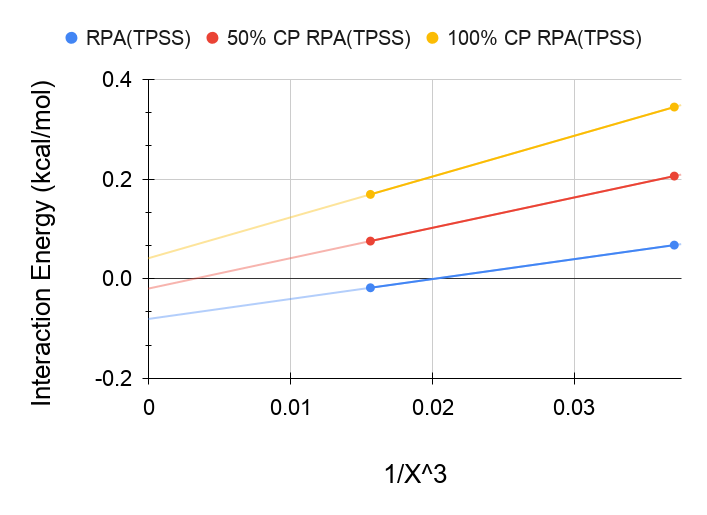
\includegraphics[scale=0.3]{tpss-1.png}
    \caption{RPA(TPSS)}
    \label{fig:tpss_1}
  \end{subfigure}%
  \begin{subfigure}{.5\textwidth}
    \centering
    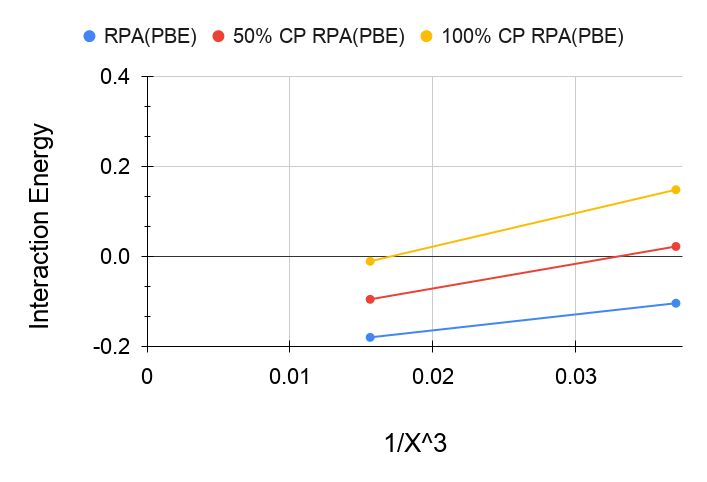
\includegraphics[scale=0.3]{tpssh-1.png}
    \caption{RPA(TPSSh)}
    \label{fig:tpssh_1}
  \end{subfigure}
  \caption{Basis sets convergence plot for RPA(TPSS) and RPA(TPSSh) is
    presented for complex 1. Dunning's basis sets were used for all atoms
    and $1/X^3$, where $X$ is the cardinal number, was used for
    extrapolation to form linear lines. Complex 1 contains dispersion
    interaction with fluorine.}
  \label{fig:complex_1}
\end{figure}

In Fig. \ref{fig:complex_1}, the convergence plot for RPA(TPSS) and
RPA(TPSSh) both don't appear to be converging since the extrapolated
lines are nearly parallel. The plot for RPA(TPSSh) also approaches a
value that is more negative than RPA(TPSS). In the previous report,
RPA(PBE) suggested that the complex 1 do not bind similar to the
RPA(TPSS). Only the RPA(TPSSh) indicates a weakly bounded complex
with 0.180 kcal/mol and this is an underestimation compared to
CCSD(T) with binding energy of 0.491 kcal/mol. The issue may due to
the MP2 geometry optimization of X40 complexes and interpolation of
the intermolecular distances using CCSD(T).

\begin{figure}[H]
  \centering
  \begin{subfigure}{.5\textwidth}
    \centering
    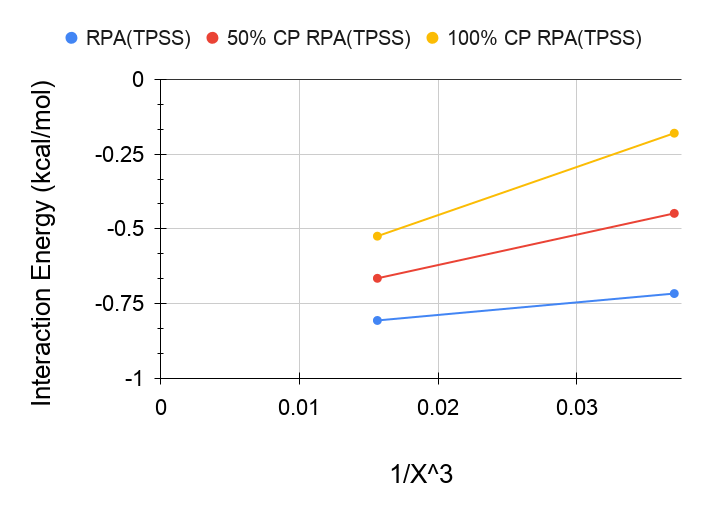
\includegraphics[scale=0.3]{tpss-8.png}
    \caption{RPA(TPSS)}
    \label{fig:tpss_8}
  \end{subfigure}%
  \begin{subfigure}{.5\textwidth}
    \centering
    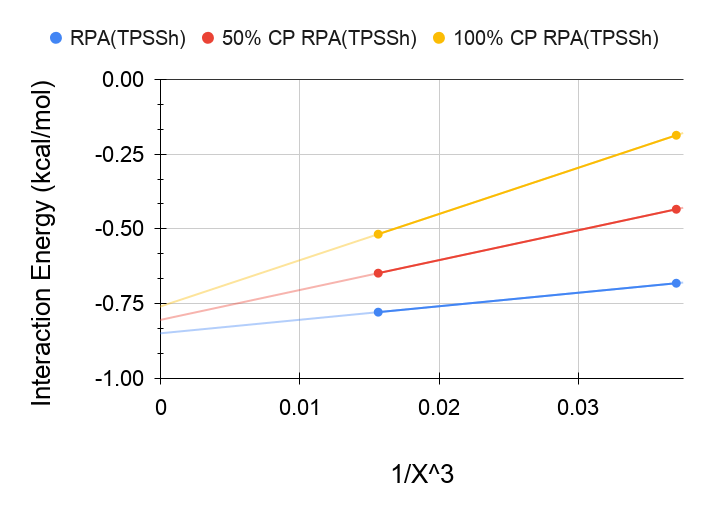
\includegraphics[scale=0.3]{tpssh-8.png}
    \caption{RPA(TPSSh)}
    \label{fig:tpssh_8}
  \end{subfigure}
  \caption{Basis sets convergence plot for RPA(TPSS) and RPA(TPSSh) is
    presented for complex 8. Dunning's basis sets were used for all atoms
    and $1/X^3$, where $X$ is the cardinal number, was used for extrapolation
    to form linear lines. Complex 8 contains induction interactions with
    chlorine.}
  \label{fig:complex_8}
\end{figure}

In Fig. \ref{fig:complex_8}, the convergence plots for RPA(TPSS)
and RPA(TPSSh) do not appear to converge. The 50$\%$ CP and 100$\%$ CP
lines are nearly parallel. RPA(TPSS) and RPA(TPSSh) underbinds with
binding energies of 0.824 kcal/mol and 0.804 kcal/mol compared to CCSD(T)
with binding energy of 1.146 kcal/mol.

\begin{figure}[hbpt]
  \centering
  \begin{subfigure}{.5\textwidth}
    \centering
    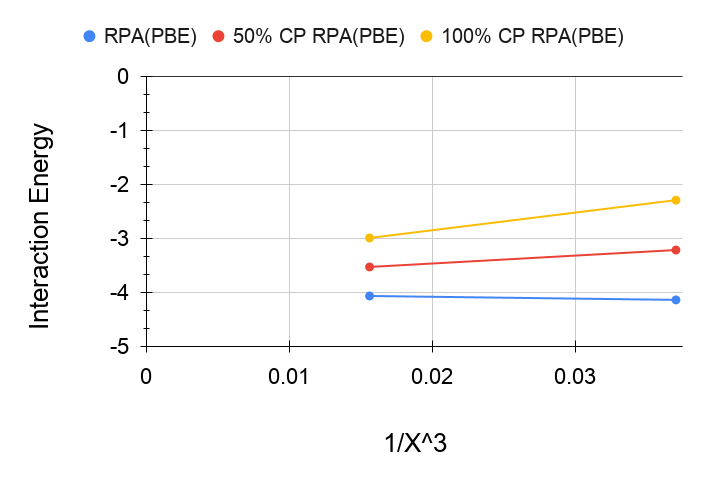
\includegraphics[scale=0.3]{tpss-11.png}
    \caption{RPA(TPSS)}
    \label{fig:tpss11}
  \end{subfigure}%
  \begin{subfigure}{.5\textwidth}
    \centering
    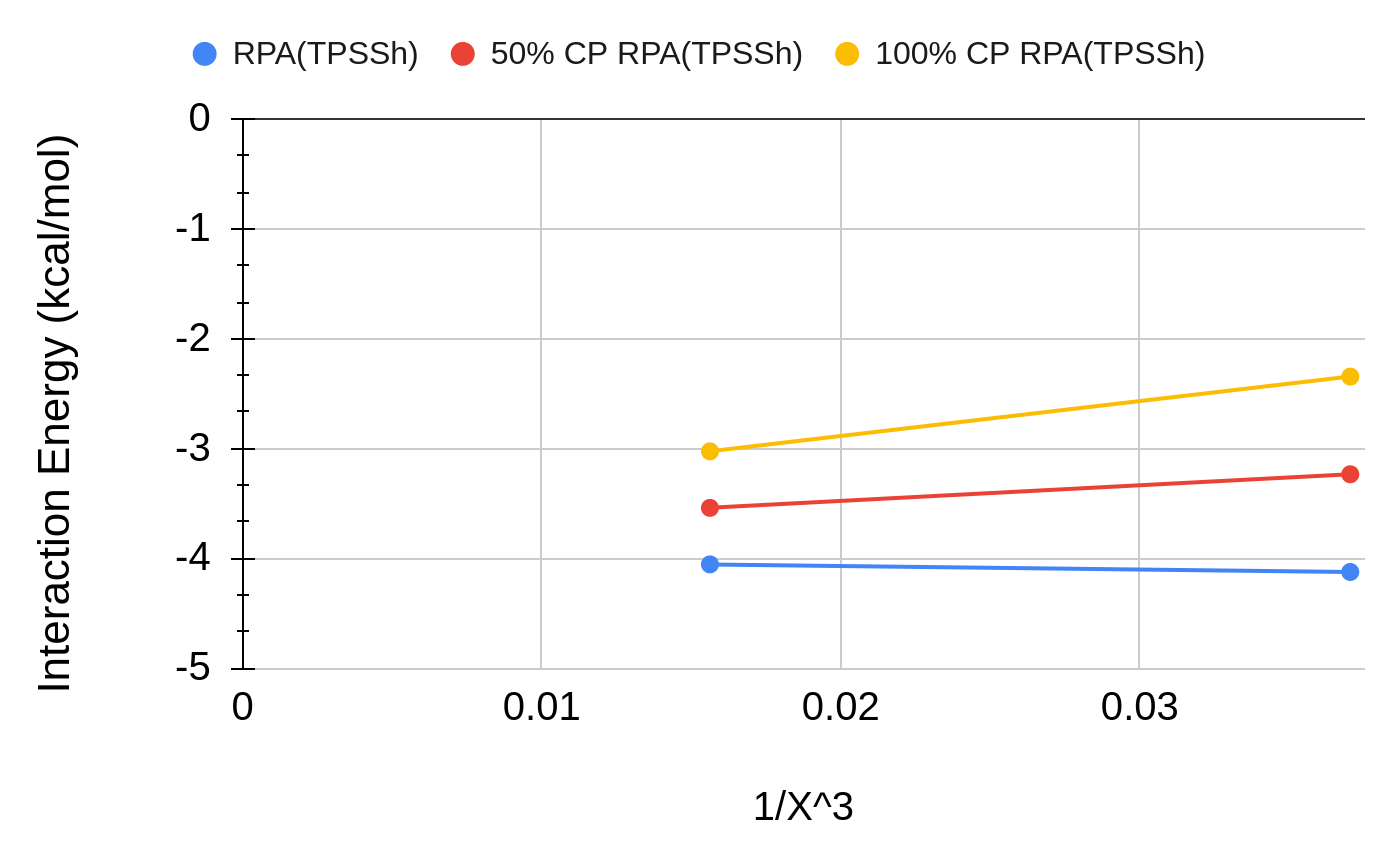
\includegraphics[scale=0.3]{tpssh-11.png}
    \caption{RPA(TPSSh)}
    \label{fig:tpssh_11}
  \end{subfigure}
  \caption{Basis sets convergence plot for RPA(TPSS) and RPA(TPSSh) is
    presented for complex 11. Dunning's basis sets were used for all
    atoms and $1/X^3$, where $X$ is the cardinal number, was used for
    extrapolation to form linear lines. Complex 11 contains stack
    interactions with fluorine.}
  \label{fig:complex_11}
\end{figure}

Both the RPA(TPSS) and RPA(TPSSh) plots for complex 11 are converging
to one value as they approach 0 in Fig. \ref{fig:complex_11}. The
interaction energy for RPA(TPSS) appears to bind while the energy
for RPA(TPSSh) suggest that complex do not bind.

\begin{figure}[H]
  \centering
  \begin{subfigure}{.5\textwidth}
    \centering
    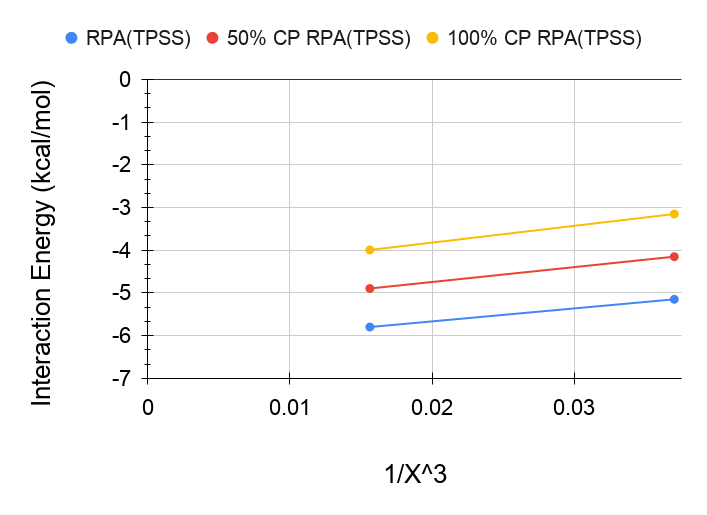
\includegraphics[scale=0.3]{tpss-24.png}
    \caption{RPA(TPSS)}
    \label{fig:tpss_24}
  \end{subfigure}%
  \begin{subfigure}{.5\textwidth}
    \centering
    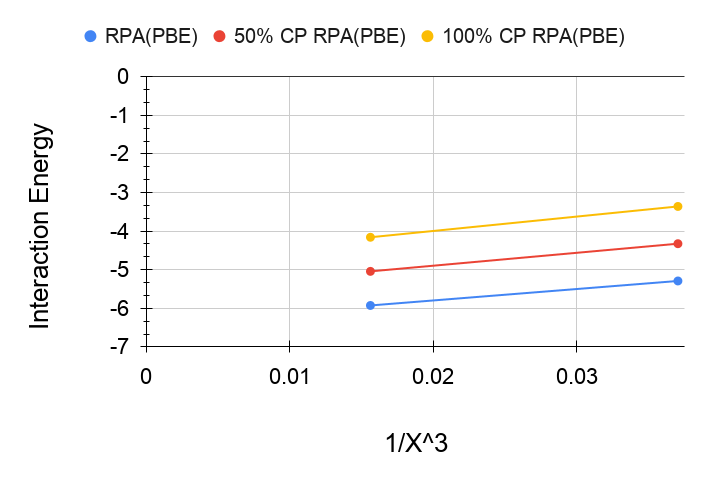
\includegraphics[scale=0.3]{tpssh-24.png}
    \caption{RPA(TPSSh)}
    \label{fig:tpssh_24}
  \end{subfigure}
  \caption{Basis sets convergence plot for RPA(TPSS) and RPA(TPSSh) is
    presented for complex 24. Dunning's basis sets were used for all
    atoms and $1/X^3$, where $X$ is the cardinal number, was used for
    extrapolation to form linear lines. Complex 24 contains halogen 
    bonding with iodine.}
  \label{fig:complex_24}
\end{figure}

The complexes containing iodine yield similar basis sets convergences
as compared to the RPA(PBE) in the previous report. Pseudo-potentials
for the iodine atom may attributed to this non-convergent behavior.
For complex 24, both RPA(TPSS) and RPA(TPSSh) do not converge at all.
The lines for both plots are parallel to each other as they approach 0.
However, the binding errors for RPA(TPSS) and RPA(TPSSh) are 0.367 kcal/mol
and 0.236 kcal/mol, respectively. The RPA(PBE) method yields a binding
error of 0.282 kcal/mol. 

\begin{figure}[hbpt]
  \centering
  \begin{subfigure}{.5\textwidth}
    \centering
    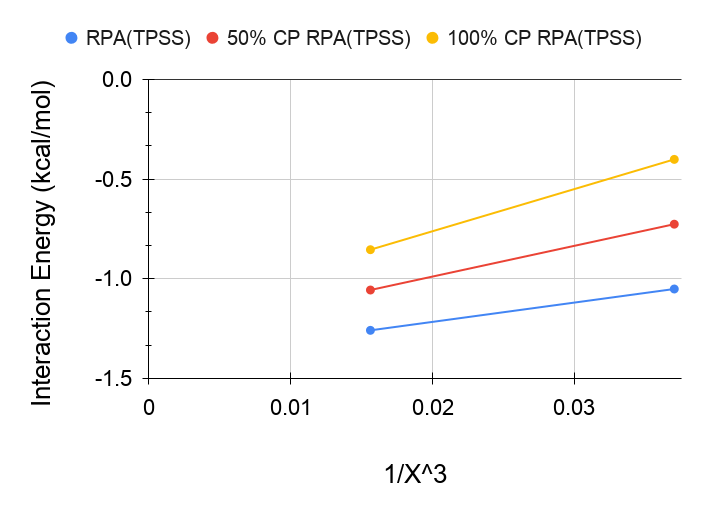
\includegraphics[scale=0.3]{tpss-27.png}
    \caption{RPA(TPSS)}
    \label{fig:tpss_27}
  \end{subfigure}%
  \begin{subfigure}{.5\textwidth}
    \centering
    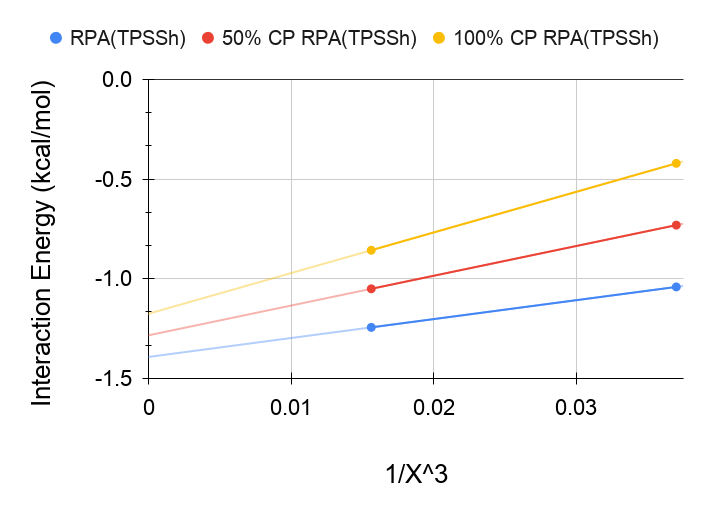
\includegraphics[scale=0.3]{tpssh-27.png}
    \caption{RPA(TPSSh)}
    \label{fig:tpssh_27}
  \end{subfigure}
  \caption{Basis sets convergence plot for RPA(TPSS) and RPA(TPSSh) is
    presented for complex 27. Dunning's basis sets were used for all
    atoms and $1/X^3$, where $X$ is the cardinal number, was used for
    extrapolation to form linear lines. Complex 27 contains halogen-$\pi$
    bonding with bromine.}
  \label{fig:complex_27}
\end{figure}

Similarly, in Fig. \ref{fig:complex_27}, the RPA(TPSS) and RPA(TPSSh)
convergence plots appear to not converge to one point. The extrapolated
lines from cc-pVTZ to cc-pVQZ appear nearly parallel with each other.
Meanwhile, the binding energy errors for RPA(PBE), RPA(TPSS), and
RPA(TPSSh) are 0.499 kcal/mol, 0.517 kcal/mol, and 0.530 kcal/mol,
respectively.

\begin{figure}[hbpt]
  \centering
  \begin{subfigure}{.5\textwidth}
    \centering
    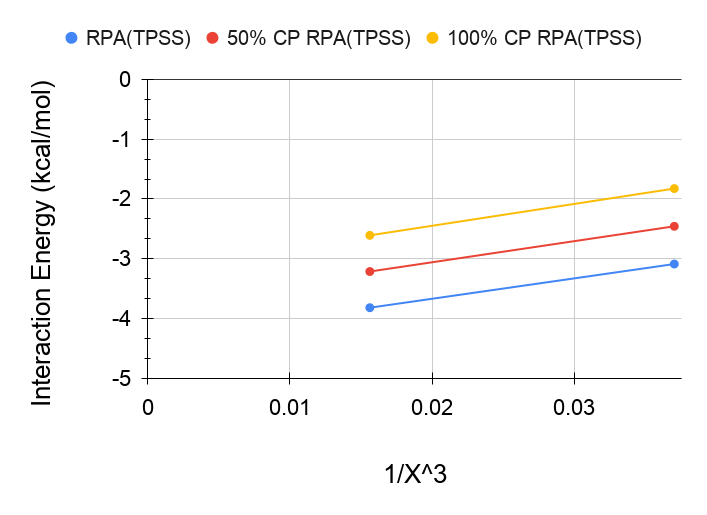
\includegraphics[scale=0.3]{tpss-30.png}
    \caption{RPA(TPSS)}
    \label{fig:tpss_30}
  \end{subfigure}%
  \begin{subfigure}{.5\textwidth}
    \centering
    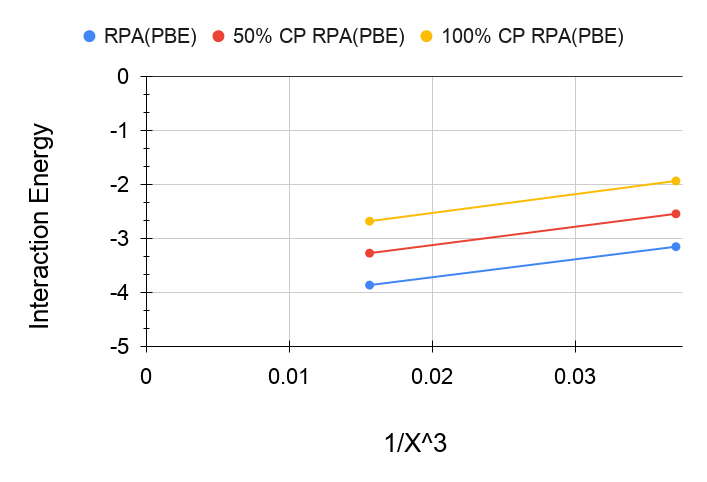
\includegraphics[scale=0.3]{tpssh-30.png}
    \caption{RPA(TPSSh)}
    \label{fig:tpssh_30}
  \end{subfigure}
  \caption{Basis sets convergence plot for RPA(TPSS) and RPA(TPSSh) is
    presented for complex 30. Dunning's basis sets were used for all
    atoms and $1/X^3$, where $X$ is the cardinal number, was used for
    extrapolation to form linear lines. Complex 30 contains halogen-$\pi$
    bonding with iodine.}
  \label{fig:complex_30}
\end{figure}

Lastly, the complex 30 convergence plot for RPA(TPSS) and RPA(TPSSh) both
do not converge as the extrapolated lines approach 0. The lines for 0$\%$,
50$\%$ CP, and 100$\%$ CP appear to be parallel. The errors for RPA(PBE),
RPA(TPSS), and RPA(TPSSh) are 0.097 kcal/mol, 0.150 kcal/mol, and 0.120
kcal/mol, respectively.

\begin{figure}[hbpt]
  \centering
  \begin{subfigure}{.5\textwidth}
    \centering
    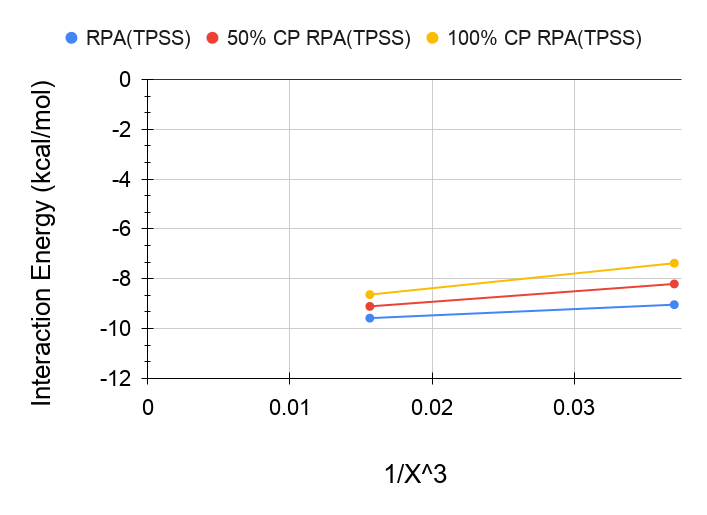
\includegraphics[scale=0.3]{tpss-38.png}
    \caption{RPA(TPSS)}
    \label{fig:tpss_38}
  \end{subfigure}%
  \begin{subfigure}{.5\textwidth}
    \centering
    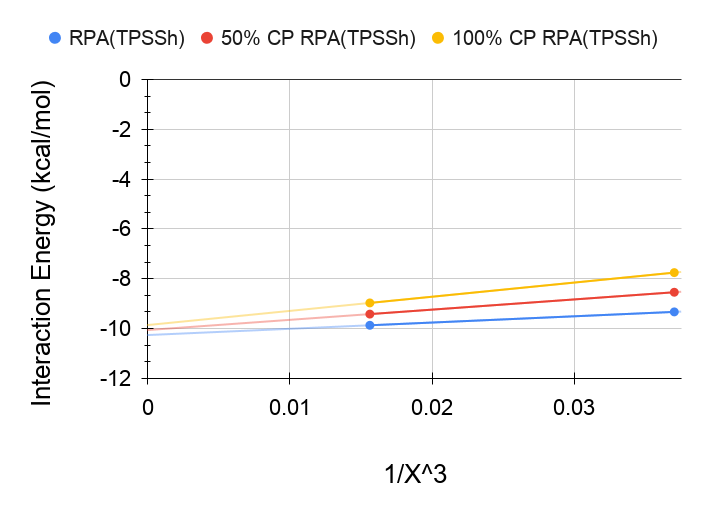
\includegraphics[scale=0.3]{tpssh-38.png}
    \caption{RPA(TPSSh)}
    \label{fig:tpssh_38}
  \end{subfigure}
  \caption{Basis sets convergence plot for RPA(TPSS) and RPA(TPSSh) is
    presented for complex 38. Dunning's basis sets were used for all
    atoms and $1/X^3$, where $X$ is the cardinal number, was used for
    extrapolation to form linear lines. Complex 38 contains hydrogen
    bonding with chlorine.}
  \label{fig:complex_38}
\end{figure}

Convergences for chlorinated complexes appear to quickly converge and
complex 38 is not exception shown in Fig. \ref{fig:complex_38}. Both
RPA(TPSS) and RPA(TPSSh) yield similar binding energies of 9.768 kcal/mol
and 10.062 kcal/mol. Hence, the errors are very different for RPA(TPSS)
and RPA(TPSSh) which are 1.650 kcal/mol and 1.357 kcal/mol, respectively.

\section{Conclusions}

After investigating the binding energy errors for the X40 test set,
def2-QZVP is revealed to be a good balance between accuracy and
efficiency. The mean error of def2-QZVP,0.603 kcal/mol, is between the
mean error of cc-pVTZ, 0.833 kcal/mol, and cc-pVQZ, 0.576 kcal/mol.
def2-QZVP yields good results compared to cc-pVTZ and cc-pVQZ since it
does not have any CP to correct BSSE.

Using TPSS and TPSSh functionals for RPA do not describe the different
interactions better than PBE. The seven complexes chosen based on error
don't show any improvements because complexes 1, 8, 24, 27, 30, and 38
did not converge. When compared to the results from the previous report,
the error of the 3-4 extrapolation of RPA(TPSS) and RPA(TPSSh) were
greater than the error of RPA(PBE). It is still recommended to use
RPA(PBE) for noncovalent calculations.


\printbibliography

\end{document}
